%%%%%%%%%%%%%%%%%%%%%%%%%%%%%%%%%%%%%%%%%%%%%%%%%%%%%%%%%%%%%%%%%%%%%%%%%%%%%%%%
%2345678901234567890123456789012345678901234567890123456789012345678901234567890
%        1         2         3         4         5         6         7         8

\documentclass[letterpaper, 10 pt, conference]{ieeeconf}  % Comment this line out if you need a4paper

%\documentclass[a4paper, 10pt, conference]{ieeeconf}      % Use this line for a4 paper

\IEEEoverridecommandlockouts                              % This command is only needed if you want to use the \thanks command

\overrideIEEEmargins                                      % Needed to meet printer requirements.

%In case you encounter the following error:
%Error 1010 The PDF file may be corrupt (unable to open PDF file) OR
%Error 1000 An error occurred while parsing a contents stream. Unable to analyze the PDF file.
%This is a known problem with pdfLaTeX conversion filter. The file cannot be opened with acrobat reader
%Please use one of the alternatives below to circumvent this error by uncommenting one or the other
%\pdfobjcompresslevel=0
%\pdfminorversion=4

% See the \addtolength command later in the file to balance the column lengths
% on the last page of the document

% The following packages can be found on http:\\www.ctan.org
%\usepackage{graphics} % for pdf, bitmapped graphics files
%\usepackage{epsfig} % for postscript graphics files
%\usepackage{mathptmx} % assumes new font selection scheme installed
%\usepackage{times} % assumes new font selection scheme installed
%\usepackage{amsmath} % assumes amsmath package installed
%\usepackage{amssymb}  % assumes amsmath package installed
\usepackage[]{graphicx}
\usepackage{balance}
\usepackage{hyperref}
\usepackage{float}
\usepackage{amsfonts}
\hypersetup{
	colorlinks   = true,  % Colour links instead of ugly boxes
	urlcolor     = black, % Colour for external hyperlinks
	linkcolor    = black, % Colour of internal links
	citecolor    = black  % Colour of citations
}
\usepackage{bm}
\usepackage{caption} %% same behavior as hypcap: links take you to images instead of captions

\title{\LARGE \bf
Optimal Control for Autonomous Drone Racing
}

\author{Aleix Paris$^{1}$% <-this % stops a space
\thanks{$^{1}$Graduate Research Assistant at the Aerospace Controls Laboratory,
        MIT, 77 Massachusetts Ave., Cambridge, MA, USA
        {\tt\small aleix@mit.edu}}%
}

\begin{document}

\maketitle
\thispagestyle{empty}
\pagestyle{empty}

%%%%%%%%%%%%%%%%%%%%%%%%%%%%%%%%%%%%%%%%%%%%%%%%%%%%%%%%%%%%%%%%%%%%%%%%%%%%%%%%

% TODO: add video and the script and world used. Add README explaining that you need a ROS package (do you, actually?), and I used ACL's.
% TODO: nu eq too big
% TODO: read sheets, they have more TODOS

\begin{abstract}

In recent years there has been interest in the subject of drone racing. This paper studies the problem of optimal control of a quadrotor to minimize the time it takes it to pass trough several waypoints, that is, to finish a race, and calculates the trajectory it will follow according to its dynamics.

\end{abstract}


%%%%%%%%%%%%%%%%%%%%%%%%%%%%%%%%%%%%%%%%%%%%%%%%%%%%%%%%%%%%%%%%%%%%%%%%%%%%%%%%
\section{INTRODUCTION}\label{s:intro}

Optimal control problems have been widely studied in literature. In particular, in the aerospace sector they proved useful in applications such as the space exploration. The Red Bull Air Race, where airplanes cross gates to end a circuit as fast as possible is another example of an optimal control problem in the aerospace industry. Nowadays, every team has the role of a `tactician', which is in charge of calculating what control inputs the pilot has to apply to their aircraft to maximize performance. This role has proved to be essential for teams to be competitive.

More recently, researchers have studied the problem of drone racing. Authors in \cite{jung2018perception} and \cite{kaufmann2018deep} apply deep learning techniques, while in \cite{jung2018direct}, authors develop a framework based on direct visual servoing and leg-by-leg planning for navigating in obstacle-dense environments as posed in the 2016 IROS Autonomous Drone Racing Challenge. In this paper, this problem is solved using the software tool GPOPS-II \cite{patterson2014gpops} with the objective to find the optimal control inputs that could allow a drone to autonomously finish a race.

The paper is structured as follows: Section~\ref{s:problem} presents the formulation of this problem, Section~\ref{s:impl} explains how this problem was implemented in GPOPS, Section~\ref{s:res} discusses the results obtained and, finally, Section~\ref{s:conclusions} concludes this paper.


\section{PROBLEM FORMULATION}\label{s:problem}

Several authors (\cite{bouabdallah2007full}, \cite{chovancova2014mathematical}, \cite{luukkonen2011modelling}, \cite{beard2008quadrotor}) have studied quadrotor dynamics. This section presents the assumptions presumed, the geometry of a quadrotor, its dynamics, the state-space model used, and the mathematical formulation of the problem in hand.

\subsection{Assumptions}

The formulation that follows considers the following assumptions:
\begin{enumerate}
	\item The maximum and minimum altitudes of the quadrotor are similar and thus the air density and gravity are constants.
	\item The vehicle is flying in zero-wind conditions.
	\item No ground effect is considered.
	\item \label{as:Ir} The angular velocities of the rotors are similar, and the rotors' inertia is small.
	\item \label{as:inertia} The quadrotor is symmetrical with its four arms aligned with the body x- and y-axes.
	\item The propellers are rigid and thus blade flapping does not occur.
\end{enumerate}

In the next subsections, the quadrotor geometry, notation and dynamics are derived, and are mostly based on \cite{luukkonen2011modelling}.

\subsection{Quadrotor Geometry and Notation}

The quadrotor's absolute linear position is defined in the inertial frame with the vector \bm{$\xi$}. Similarly, the attitude (angular position of the drone with respect to the inertial frame) is defined with the vector \bm{$\eta$}. Roll angle $\phi$ determines the rotation of the vehicle around the x-axis, pitch angle $\theta$ defines a rotation around the y-axis, and yaw angle $\psi$ determines the quadrotor's rotation around the z-axis:


$$\bm{\xi}=\left[ \begin{array}{l}{x} \\ {y} \\ {z}\end{array}\right],
\quad \bm{\eta}=\left[ \begin{array}{l}{\phi} \\ {\theta} \\ {\psi}\end{array}\right]$$

The origin of the body frame, indicated with a B, is the center of mass of the quadrotor. In this frame, the vehicle's linear velocities \bm{$V_B$} and angular velocities \bm{$\nu$} are:

$$\bm{V}_{B}=\left[ \begin{array}{c}{v_{x, B}} \\ {v_{y, B}} \\ {v_{z, B}}\end{array}\right], \quad \bm{\nu}=\left[ \begin{array}{l}{p} \\ {q} \\ {r}\end{array}\right]$$

Figure~\ref{fig:quad_frame} shows the inertial and body frame, as well as the Euler and angular velocity angles defined previously.

\begin{figure}[!htpb]
	\centering
	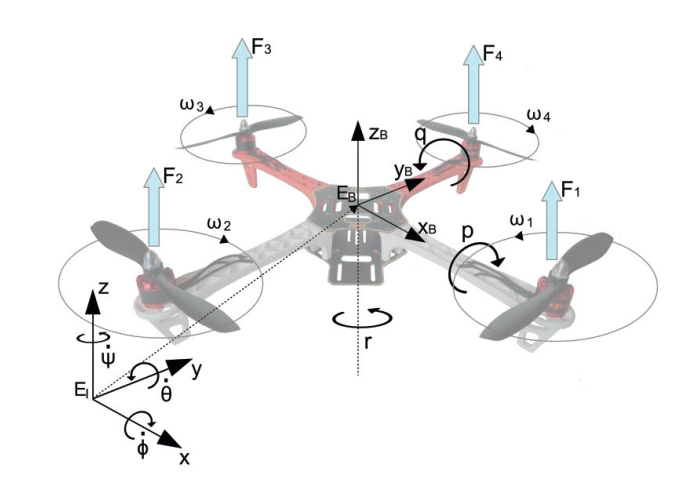
\includegraphics[width=1.0\linewidth]{Images/quad_frame.png}
	\caption{Inertial and body-fixed frame of the quadrotor, showing the Euler and angular velocity angles [?] %TODO CITE Mathematical modelling and...
		}
	\label{fig:quad_frame}
\end{figure}


 The rotation from the body frame to the inertial frame can be defined with the matrix

$$\bm{R}=\left[ \begin{array}{ccc}{C_{\psi} C_{\theta}} & {C_{\psi} S_{\theta} S_{\phi}-S_{\psi} C_{\phi}} & {C_{\psi} S_{\theta} C_{\phi}+S_{\psi} S_{\phi}} \\ {S_{\psi} C_{\theta}} & {S_{\psi} S_{\theta} S_{\phi}+C_{\psi} C_{\phi}} & {S_{\psi} S_{\theta} C_{\phi}-C_{\psi} S_{\phi}} \\ {-S_{\theta}} & {C_{\theta} S_{\phi}} & {C_{\theta} C_{\phi}}\end{array}\right]$$

in which $S_{x}=\sin (x)$ and $C_{x}=\cos (x)$. Note that this rotation matrix is orthogonal and thus the rotation matrix from the inertial frame to the body frame is $\bm{R^{-1} = \bm{R^T}}$.

To obtain the angular velocities in the body frame from the angular velocities in the inertial frame, the matrix $\bm{W_\eta}$ should be used:

$\bm{\nu}=\bm{W}_{\eta} \dot{\bm{\eta}}, \hfill \left[ \begin{array}{l}{p} \\ {q} \\ {r}\end{array}\right]=\left[ \begin{array}{ccc}{1} & {0} & {-S_{\theta}} \\ {0} & {C_{\phi}} & {C_{\theta} S_{\phi}} \\ {0} & {-S_{\phi}} & {C_{\theta} C_{\phi}}\end{array}\right] \left[ \begin{array}{c}{\dot{\phi}} \\ {\dot{\theta}} \\ {\dot{\psi}}\end{array}\right]$

Its inverse is the transformation matrix from the body frame to the inertial frame, which will be used later to assemble the quadrotor dynamics:

$\dot{\bm{\eta}}=\bm{W}_{\eta}^{-1} \bm{\nu}$, \hfill $\left[ \begin{array}{c}{\dot{\phi}} \\ {\dot{\theta}} \\ {\dot{\psi}}\end{array}\right]=\left[ \begin{array}{ccc}{1} & {S_{\phi} T_{\theta}} & {C_{\phi} T_{\theta}} \\ {0} & {C_{\phi}} & {-S_{\phi}} \\ {0} & {S_{\phi} / C_{\theta}} & {C_{\phi} / C_{\theta}}\end{array}\right] \left[ \begin{array}{l}{p} \\ {q} \\ {r}\end{array}\right]$

where $T_{x}=\tan (x)$.

As shown in Figure~\ref{fig:quad_frame} and stated in assumption~\ref{as:inertia}, the drone is symmetric with the arms aligned with the body axes. Therefore, the inertia matrix $\textbf{I}$ is diagonal, and $I_{xx} = I_{yy}$:

 $$\bm{I}=\left[ \begin{array}{ccc}{I_{x x}} & {0} & {0} \\ {0} & {I_{y y}} & {0} \\ {0} & {0} & {I_{z z}}\end{array}\right]$$
 
 \subsection{Quadrotor Dynamics}

The force $f_i$ created by the angular velocity of rotor $i$, denoted with $\omega_i$, in the direction of the rotor axis is:

$$f_{i}=k \omega_{i}^{2}$$

Additionally, torque $\tau_{M_i}$ is created around the rotor axis:

$$\tau_{M_{i}} = b \omega_{i}^{2} + I_{r} \dot{\omega}_{i} $$

where the lift constant is $k$, the drag constant is $b$ and the inertia moment of the rotor is $I_{r}$. As assumption~\ref{as:Ir} considered, the rotor's inertia is small, and $\dot{\omega}_{i}$ is also usually small. Therefore, this term can be omitted.

The rotors create thrust $T$ in the direction of the body z-axis, and torque $\bm{\tau_B}$ consists of torques $\tau_\phi, \tau_\theta, \tau_\psi$ in the direction of the corresponding body frame angles:

$$T=\sum_{i=1}^{4} f_{i}=k \sum_{i=1}^{4} \omega_{i}^{2}, \quad \quad \bm{T}^{B}=\left[ \begin{array}{c}{0} \\ {0} \\ {T}\end{array}\right]$$

$$
\bm{\tau}_{B}=\left[ \begin{array}{c}{\tau_{\phi}} \\ {\tau_{\theta}} \\ {\tau_{\psi}}\end{array}\right]=
\left[ \begin{array}{c}{l k\left(-\omega_{2}^{2}+\omega_{4}^{2}\right)} \\ {l k\left(-\omega_{1}^{2}+\omega_{3}^{2}\right)} \\ {\sum_{i=1}^{4} \tau_{M_{i}}}\end{array}\right]
$$

in which l is the distance between the rotor and the center of mass of the quadcopter.

The Newton-Euler equations for the quadrotor are:

$$m \ddot{\bm{\xi}}=\bm{G}+\bm{R} \bm{T}_{B}$$

$$\left[ \begin{array}{c}{\ddot{x}} \\ {\ddot{y}} \\ {\ddot{z}}\end{array}\right]=-g \left[ \begin{array}{l}{0} \\ {0} \\ {1}\end{array}\right]+\frac{T}{m} \left[ \begin{array}{c}{C_{\psi} S_{\theta} C_{\phi}+S_{\psi} S_{\phi}} \\ {S_{\psi} S_{\theta} C_{\phi}-C_{\psi} S_{\phi}} \\ {C_{\theta} C_{\phi}}\end{array}\right]$$

where g is Earth's gravity, 9.81 $m/s^2$. Additionally:
 $$\boldsymbol{I} \dot{\boldsymbol{\nu}}+\boldsymbol{\nu} \times(\boldsymbol{I} \boldsymbol{\nu})+\mathbf{\Gamma}=\boldsymbol{\tau_B}$$
 
 $$\boldsymbol{\dot{\nu}}=\boldsymbol{I}^{-1}\left(-\left[ \begin{array}{c}{p} \\ {q} \\ {r}\end{array}\right] \times \left[ \begin{array}{c}{I_{x x} p} \\ {I_{y y} q} \\ {I_{z z} r}\end{array}\right]-I_{r} \left[ \begin{array}{c}{p} \\ {q} \\ {r}\end{array}\right] \times \left[ \begin{array}{c}{0} \\ {0} \\ {1}\end{array}\right] \omega_{\Gamma}+\boldsymbol{\tau_B}\right)$$
 
 $$
 \begin{array}{c}
 \left[ \begin{array}{c}{\dot{p}} \\ {\dot{q}} \\ {\dot{r}}\end{array}\right]= 
 \left[ \begin{array}{c}{\left(I_{y y}-I_{z z}\right) q r / I_{x x}} \\ {\left(I_{z z}-I_{x x}\right) p r / I_{y y}} \\ {(I_{x x}-I_{y y}) p q / I_{z z}}\end{array}\right] 
 - I_{r} \left[ \begin{array}{c}{q / I_{x x}} \\ {-p / I_{y y}} \\ {0}\end{array}\right] \omega_{\Gamma} \\
 + \left[ \begin{array}{c}{\tau_{\phi} / I_{x x}} \\ {\tau_{\theta} / I_{y y}} \\ {\tau_{\psi} / I_{z z}}\end{array}\right]
 \end{array}
 $$
 
 where $\omega_\Gamma = \omega_1 - \omega_2 + \omega_3 - \omega_4$. By assumption~\ref{as:Ir}, the term that includes $I_r$ and $\omega_\Gamma$ can be omitted.
 
 Finally, this work considers aerodynamic drag caused by the vehicle's translation. Therefore, the revised Netwon equation is:
 
  $$
  \begin{array}{l}
  \left[ \begin{array}{l}{\ddot{x}} \\ {\ddot{y}} \\ {\ddot{z}}\end{array}\right]=-g \left[ \begin{array}{l}{0} \\ {0} \\ {1}\end{array}\right]+\frac{T}{m} \left[ \begin{array}{c}{C_{\psi} S_{\theta} C_{\phi}+S_{\psi} S_{\phi}} \\ {S_{\psi} S_{\theta} C_{\phi}-C_{\psi} S_{\phi}} \\ {C_{\theta} C_{\phi}}\end{array}\right] \\
  \quad \quad \quad \quad  - \frac{1}{m} \left[ \begin{array}{ccc}{A_{x}} & {0} & {0} \\ {0} & {A_{y}} & {0} \\ {0} & {0} & {A_{z}}\end{array}\right] \left[ \begin{array}{c}{\dot{x}} \\ {\dot{y}} \\ {\dot{z}}\end{array}\right]
  \end{array}
  $$
  
  where $A_x, A_y$, and $A_z$ are the drag force coefficients for velocities in the corresponding directions of the inertial frame.
 
\subsection{State-space Representation}

The state of the quadrotor can be represented as follows:

 $$ \bm{X} = \left[ 
 \begin{array}{c}
  {\bm{x}}  \\
  {\bm{\dot{x}}}  \\
  {\bm{\eta}}  \\
  {\bm{\nu}}
  \end{array}\right]$$

that is, a column vector of $4 \cdot 3 = 12$ components that contains the inertial position, the inertial velocity, the Euler angles and the angular velocities in the body frame. The control inputs are:

 $$ \bm{U} = \left[ 
 \begin{array}{c}
 {T}  \\
 {\tau_\phi}  \\
 {\tau_\theta}  \\
 {\tau_\psi}
 \end{array}\right]$$
 
 that is, the total thrust $T$ and the torques $\tau$ that cause a roll, pitch, and yaw angle change, respectively.
 
 The dynamics previously derived can be assembled in vector $\bm{\dot{X}} = f(\boldsymbol{X}, \boldsymbol{U})$, which represents the change of the state as a function of the state and the inputs. That is:
 
 $$
 \dot{\boldsymbol{X}} =
 \left[
 \begin{array}{c}
 \dot{x} \\
 {}\\
 \dot{y} \\
 {}\\
 \dot{z} \\
 {}\\
 {}\\
 \ddot{x} \\
 {}\\
 \ddot{y} \\
 {}\\
 \ddot{z} \\
 {}\\
 {}\\
 \dot{\phi} \\
 {}\\
 \dot{\theta} \\
 {}\\
 \dot{\psi} \\
 {}\\
 {}\\
 \dot{p} \\
 {}\\
 \dot{q} \\
 {}\\
 \dot{r}
 \end{array}
 \right]
 =
 \left[
 \begin{array}{l}
 \dot{x} \\
 {}\\
 \dot{y} \\
 {}\\
 \dot{z} \\
 {}\\
 {}\\
 \frac{T}{m}[C_{\psi} S_{\theta} C_{\phi} + S_{\psi} S_{\phi}] - \frac{A_x}{m} \dot{x} \\
 {}\\
 \frac{T}{m}[ S_{\psi} S_{\theta} C_{\phi} - C_{\psi} S_{\phi}] - \frac{A_y}{m} \dot{y} \\
 {}\\
 -g+\frac{T}{m}[C_{\theta} C_{\phi}] - \frac{A_z}{m} \dot{z} \\
 {}\\
 {}\\
 p+ q[S_{\phi} T_{\theta}] + r[C_{\phi} T_{\theta}] \\
 {}\\
 q[C_{\phi}]-r[S_{\phi}] \\
 {}\\
 q \frac{S_{\phi}}{C_{\theta}} + r \frac{C_{\phi}}{C_{\theta}} \\
 {}\\
 {}\\
 \frac{I_{yy}-I_{zz}}{I_{xx}} q r  +\frac{\tau_{\phi}}{I_{xx}} \\
 {}\\
 \frac{I_{zz}-I_{xx}}{I_{yy}} p r +\frac{\tau_{\theta}}{I_{yy}} \\
 {}\\
 \frac{I_{xx}-I_{yy}}{I_{zz}} p q +\frac{\tau_{\psi}}{I_{zz}}
 \end{array}
 \right]
 $$

\subsection{Mathematical Formulation}\label{subs:math_form}
The problem in hand consists of minimizing the time a drone takes to complete a race, that is, to cross all the gates in a specific order as fast as possible. In this paper, the gates are considered point constraints only, and it does not matter the direction of the velocity vector. This can be formulated mathematically as an optimal control problem:

\bigskip

Minimize \quad $\int_{t_0}^{t_f} 1 dt = \int_{0}^{t_f} 1 dt = t_f$

\bigskip

subject to:

$$ \bm{\dot{X}} = f(\boldsymbol{X}, \boldsymbol{U}) $$

$$ \bm{X}(0) = 0 $$

\quad $ \bm{x}(t_i) = \bm{g_i},$ \quad $t_i < t_{i+1} $ for $i = 1 .. n_{gates}-1$

$$ z \ge 0 $$

$$ 0 \le T \le T_{max} $$
$$  |\tau_{\phi}| \le \tau_{\phi,max} $$
$$  |\tau_{\theta}| \le \tau_{\theta,max} $$
$$  |\tau_{\psi}| \le \tau_{\psi,max} $$

The first constraint imposes the quadrotor dynamics. The second one, states that the initial state of the drone is 0, that is, the drone is stopped in the origin and the body axes match the global axes. The third constraint are the gates: the drone's position $\bm{x}$ has to match the gates' positions $\bm{g_i}$ in increasing times (that is, the gates have to be crossed in order, from number 1 to number $n_{gates}$). The next constraint ensures that the drone will not crash against the ground. The last four constraints limit the control inputs, necessary to account for the limitations of the quadrotor's propellers and motors.

\section{PROBLEM IMPLEMENTATION}\label{s:impl}

The problem was implemented in GPOPS-II \cite{patterson2014gpops}, a MATLAB software to solve optimal control problems. As shown in GPOPS-II's User Guide \cite{gpops_guide}, a program must have three main functions: the main, the continuous and the endpoint function, which are explained in the following subsections.

To specify the gate constraints, the program is divided in $n_{gates}$ phases. The first phase is from the initial state (where all the states are 0) to the first gate, the second phase is from the end of the first phase to the second gate, and so on.

\subsection{Main Function}
In this function, the race and drone parameters are loaded, the program is set up and the bounds and guesses are specified:
\begin{itemize}
	\item \textbf{Bounds:} the bounds limit the states and controls allowed for each phase. The time, position, velocity, orientation and rates are limited to realistic values, although the quadrotor could technically surpass them. For example, this work does not allow the drone to fly faster than 50 $m/s$. As for the control inputs, they are limited to the allowed values as shown in Subsection~\ref{subs:math_form}.
	
	Additionally, the z is limited to values greater than 0 to avoid the drone crashing into the ground, the initial state is set to 0, the difference of states in contiguous phases is set to 0 and the final position for each phase is set to the corresponding gate. To avoid having redundant constraints, the initial positions of each phase are not set to the previous gate.
	\item \textbf{Guesses:} they set values to the time, state and control for each phase to help the algorithm converge.
\end{itemize}

Finally, the data is saved and plotted using auxiliary functions.

\subsection{Continuous Function}

This function contains all the dynamics explained in Section~\ref{s:problem}. For every phase, $\bm{\dot{X}}$ is computed and returned. Additionally, the path constraint variable is returned, that is, the state $z$. As mentioned before, its minimum is set to 0 using the lower and upper path constraint bounds.

\subsection{Endpoint Function}

The endpoint function returns the objective function, which is the final time of the last phase, and also returns the difference of the states and times between contiguous phases as something called `eventgroup'. This difference is set to 0 by the bounds, like previously explained.

\subsection{Video Functions}\label{subs:video}

To make the video of the drone performing the race, the time, position and orientation vectors obtained with GPOPS were saved to an Excel file, which was read by a Python script. Using ROS \cite{quigley2009ros}, the script publishes topics from which Gazebo \cite{koenig2004design} (a simulation environment for ROS) is subscribed. These topics include the position and orientation of the drone, and are published with a period that matches the time difference of every point. A quadrotor model in Gazebo receives the ROS messages and moves and rotates as they indicate, thus giving the impression that the drone is moving. Cuboids were added to the environment to represent the gates.


\section{RESULTS}\label{s:res}

\subsection{Quadrotor Parameters}

The following quadrotor parameters were used:

\begin{table}[!htpb]
	\caption[Quadrotor parameters]{\bf Quadrotor parameters}
	\label{tbl:drone-params}
	\centering
	\def\arraystretch{1.3}
	\setlength{\tabcolsep}{3pt}
	\begin{tabular}{ccc}
		%\specialrule{.1em}{.05em}{.00em} 
		%\rowcolor{Gray}
		\textbf{Parameter} & \textbf{Value} & \textbf{Unit} \\ 
		\hline
		Mass & 1.1 & $kg$ \\
		$I_{xx}$  & 0.03 & $kg \cdot m^2$  \\
		$I_{yy}$  & 0.03 & $kg \cdot m^2$  \\
		$I_{zz}$  & 0.16 & $kg \cdot m^2$  \\
		$A_x$     & 0.10 & $kg / s$  \\
		$A_y$     & 0.10 & $kg / s$  \\
		$A_z$     & 0.20 & $kg / s$  \\
		$T_{max}$ & 25   & $N$  \\
		$\tau_{\phi, max}$   & 5    & $ rad/s^2 \cdot kg \cdot m^2$  \\
		$\tau_{\theta, max}$ & 5    & $ rad/s^2 \cdot kg \cdot m^2$  \\
		$\tau_{\psi, max}$   & 1.5  & $ rad/s^2 \cdot kg \cdot m^2$  \\		
	%	\specialrule{.1em}{.05em}{.00em} 
	\end{tabular}
\end{table}

\subsection{Experiments}

\subsubsection{Simple experiment without the z constraint}
At first, a simple experiment was tried where the drone had to go from the origin to a gate located in $g_1=(1, 0, 0.5)$ and where the altitude was not limited to values greater or equal than zero. Figures~\ref{fig:simple_zfree_3d} to~\ref{fig:simple_zfree_controls} show the results obtained: a 3D plot of the trajectory, the 12 states over time and the control inputs over time. The 3D plot and the positions over time show the initial state marked with a dot, and the gates marked with a circle (just one in this case). As it can be seen, at first the thrust is 0 while the pitch control input is the maximum, and the drone falls to z = -0.2. Then, the trust is set to the maximum value and the drone accelerates as fast as possible, as expected. It is interesting to observe that the roll and yaw rates are not zero (actually, the drone moves 5 cm to the direction of positive y). A possible explanation is the difference between the inertia in the x- and y- axis and the inertia in the z-axis.

The decrease of the altitude below 0 is, of course, unrealistic. The following case solves this issue.

\begin{figure}[!htpb]
	\centering
	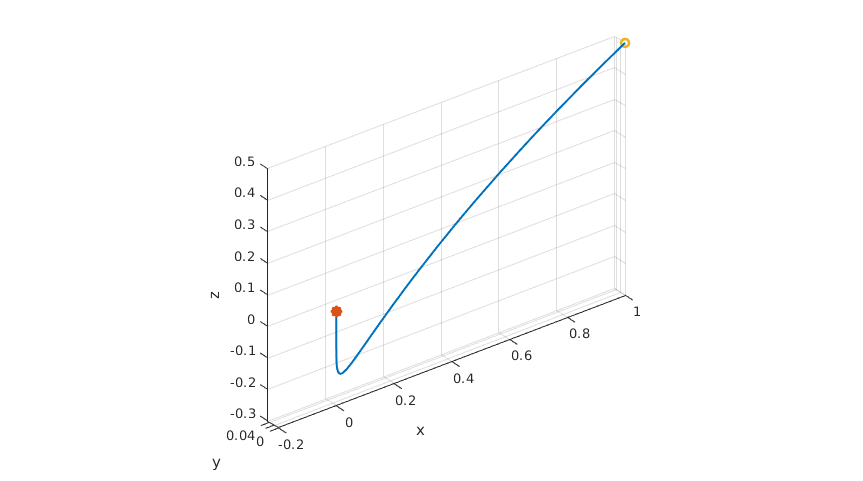
\includegraphics[width=1.0\linewidth]{Images/simple_zfree/3d.png}
	\caption{3D plot of the simple experiment without the z constraint}
	\label{fig:simple_zfree_3d}
\end{figure}
\begin{figure}[!htpb]
	\centering
	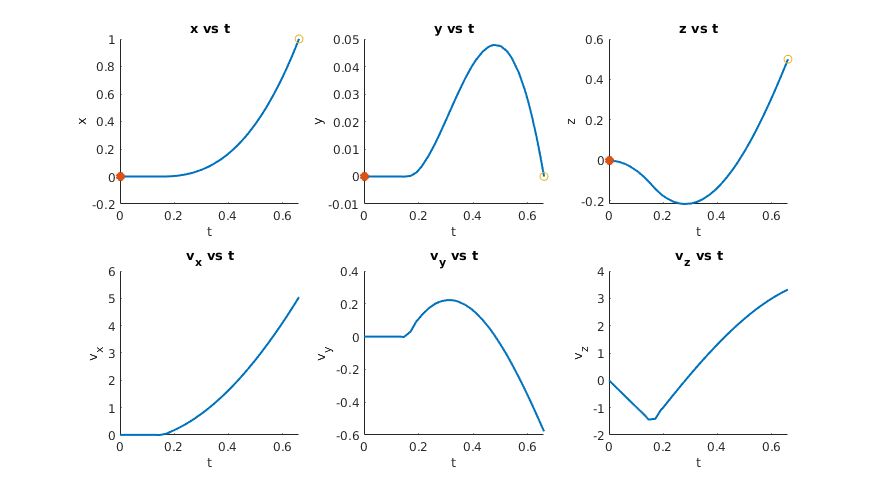
\includegraphics[width=1.0\linewidth]{Images/simple_zfree/pos_vel.png}
	\caption{Position and velocity plot of the simple experiment without the z constraint}
	\label{fig:simple_zfree_pos_vel}
\end{figure}
\begin{figure}[!htpb]
	\centering
	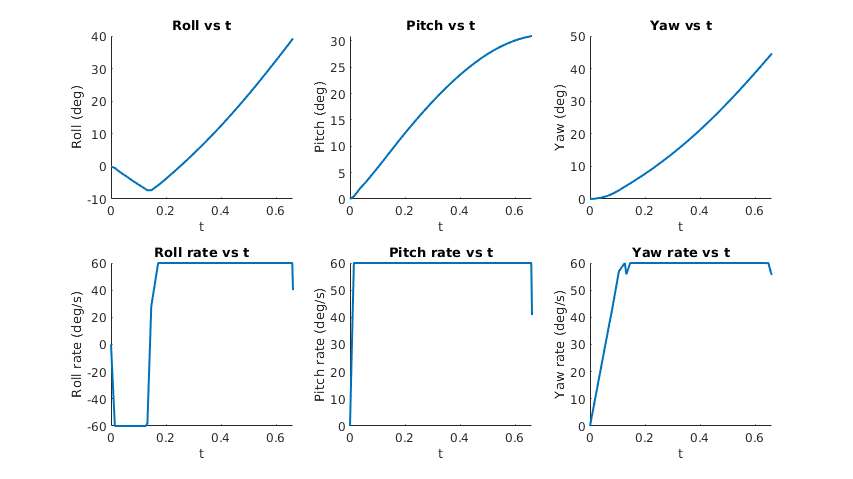
\includegraphics[width=1.0\linewidth]{Images/simple_zfree/orient_rates.png}
	\caption{Orientation and angular rates plot of the simple experiment without the z constraint}
	\label{fig:simple_zfree_orient_rates}
\end{figure}
\begin{figure}[!htpb]
	\centering
	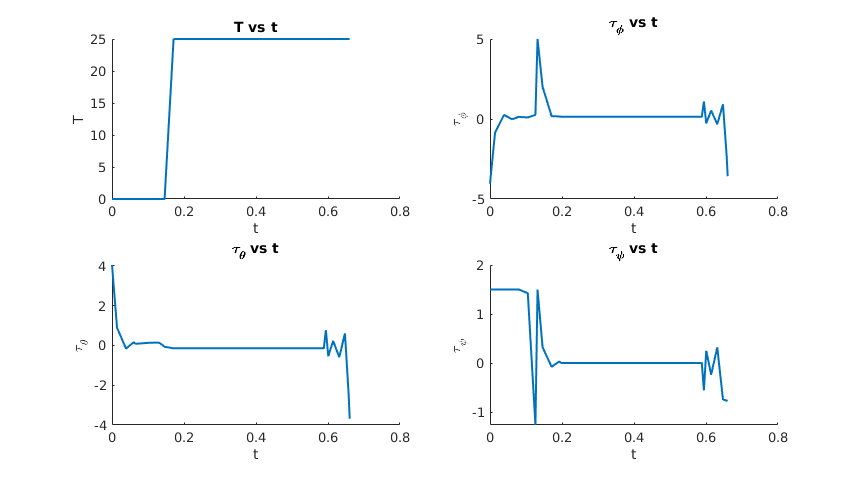
\includegraphics[width=1.0\linewidth]{Images/simple_zfree/controls.png}
	\caption{Control inputs plot of the simple experiment without the z constraint}
	\label{fig:simple_zfree_controls}
\end{figure}

\subsubsection{Simple experiment with z constraint}

In this experiment there is only one gate $g_1=(1, 0, 0.5)$ located in the same place as in the previous case, but now it is imposed that $ z \ge 0$. Figures~\ref{fig:simple_zconstr_3d} to~\ref{fig:simple_zconstr_controls} show the results that were obtained.

In this case, at first the drone applies an average thrust of roughly $mg = 10.8$ N, that is, the thrust needed to hover, while it pitches forward. Therefore, the z is maintained during the first moments and then increases similarly as before. % TODO EXPAND?

\begin{figure}[!htpb]
	\centering
	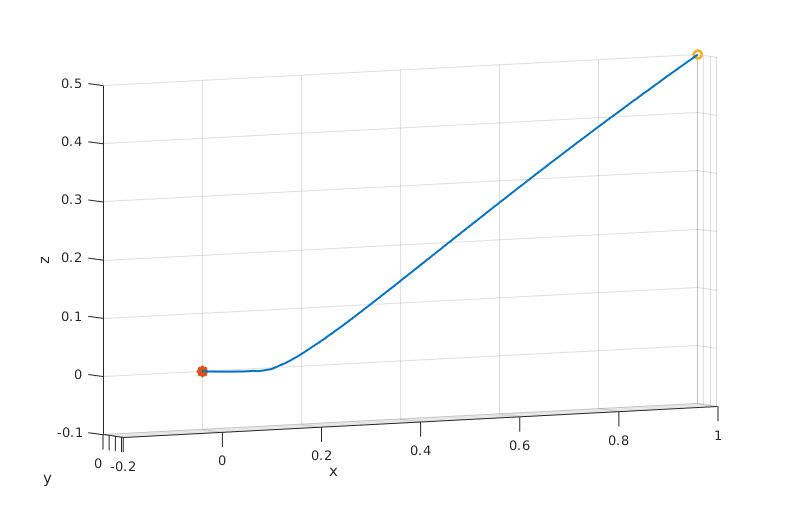
\includegraphics[width=1.0\linewidth]{Images/simple_zconstr/3d.png}
	\caption{3D plot of the simple experiment with the z constraint}
	\label{fig:simple_zconstr_3d}
\end{figure}
\begin{figure}[!htpb]
	\centering
	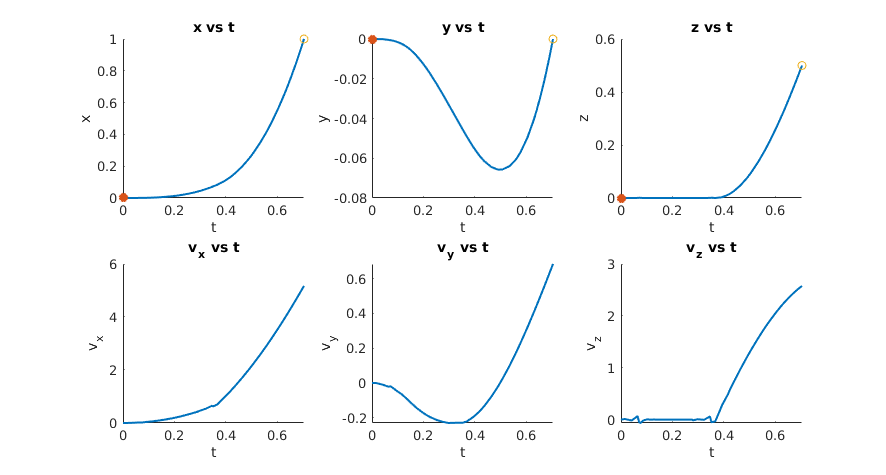
\includegraphics[width=1.0\linewidth]{Images/simple_zconstr/pos_vel.png}
	\caption{Position and velocity plot of the simple experiment with the z constraint}
	\label{fig:simple_zconstr_pos_vel}
\end{figure}
\begin{figure}[!htpb]
	\centering
	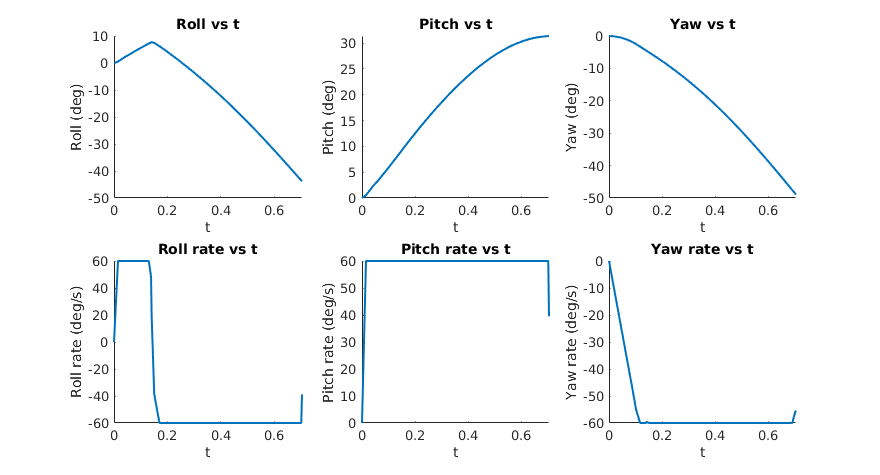
\includegraphics[width=1.0\linewidth]{Images/simple_zconstr/orient_rates.png}
	\caption{Orientation and angular rates plot of the simple experiment with the z constraint}
	\label{fig:simple_zconstr_orient_rates}
\end{figure}
\begin{figure}[!htpb]
	\centering
	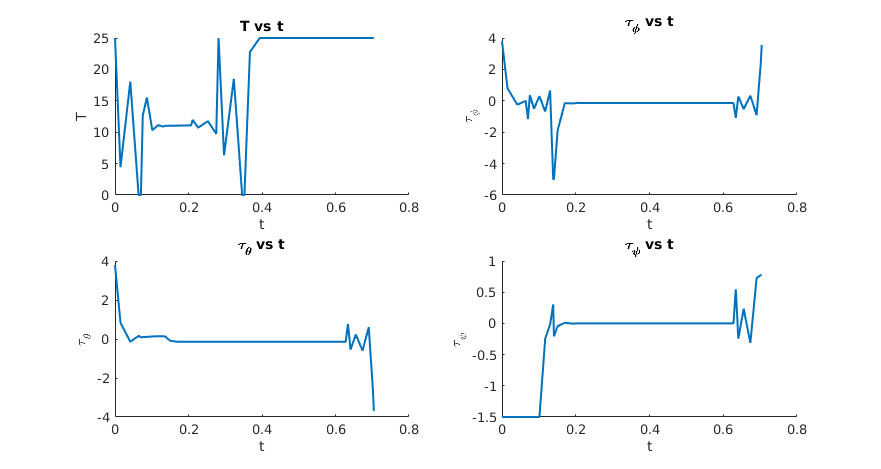
\includegraphics[width=1.0\linewidth]{Images/simple_zconstr/controls.png}
	\caption{Control inputs plot of the simple experiment with the z constraint}
	\label{fig:simple_zconstr_controls}
\end{figure}

\subsubsection{Complex experiment}

This experiment considers the z constraint explained before and has multiple gates to represent a real drone race. The gates are indicated in Table~\ref{tbl:gates}. The initial position is, as always, the origin. Figures~\ref{fig:final_3d} to~\ref{fig:final_controls} show the results obtained. The variables over time are plotted a different color for each phase.

\begin{table}[!htpb]
	\caption[Gates]{\bf Gates for the complex experiment}
	\label{tbl:gates}
	\centering
	\def\arraystretch{1.3}
	\setlength{\tabcolsep}{3pt}
	\begin{tabular}{cccc}
		%\specialrule{.1em}{.05em}{.00em} 
		%\rowcolor{Gray}
		\textbf{Gate} & \textbf{x} & \textbf{y} & \textbf{z} \\ 
		\hline
		$g_1$ & 1 & 0 & 1 \\ 
		$g_2$ & 1 & 1 & 1 \\ 
		$g_3$ & 3 & 2 & 3 \\ 
		$g_4$ & 3 & 1 & 1 \\ 
		$g_5$ & 5 & 0 & 1 \\ 
	\end{tabular}
\end{table}

The trajectory observed in Figure~\ref{fig:final_3d} shows what it could be thought intuitively. In the end of the first phase (from the origin to $g_1$), the quadrotor rolls and pitches to change its velocity to the left, where the second gate is. This kind of anticipation just before going through a gate is characteristic of car and airplane races, and drone racing is not an exception. After going to the second gate with considerable $v_y$, the drone ascends to the third gate, sets the thrust to zero for some seconds to free-fall to the forth gate (2 meters below it and 1 meter to the right) and, finally, it sets its thrust to the maximum until the end to do the final straight leg, finishing at a $v_x$ of almost 8 $m/s$. % TODO EXPAND?

\begin{figure}[!htpb]
	\centering
	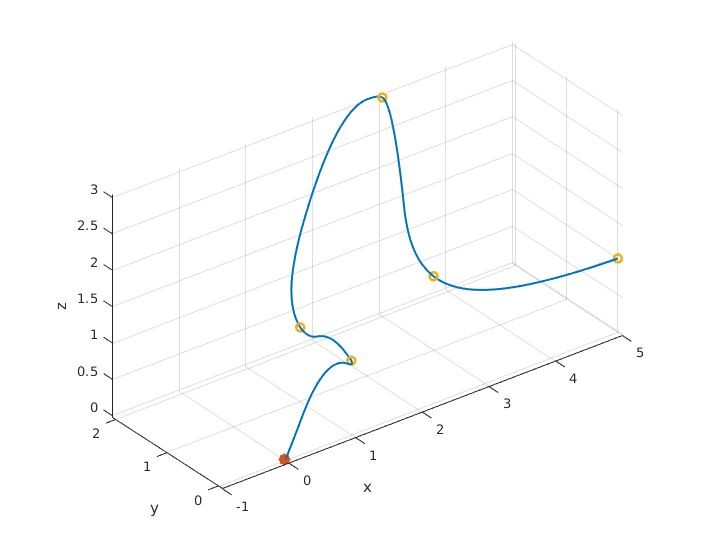
\includegraphics[width=1.0\linewidth]{Images/final_race/3d.png}
	\caption{3D plot of the complex experiment}
	\label{fig:final_3d}
\end{figure}
\begin{figure}[!htpb]
	\centering
	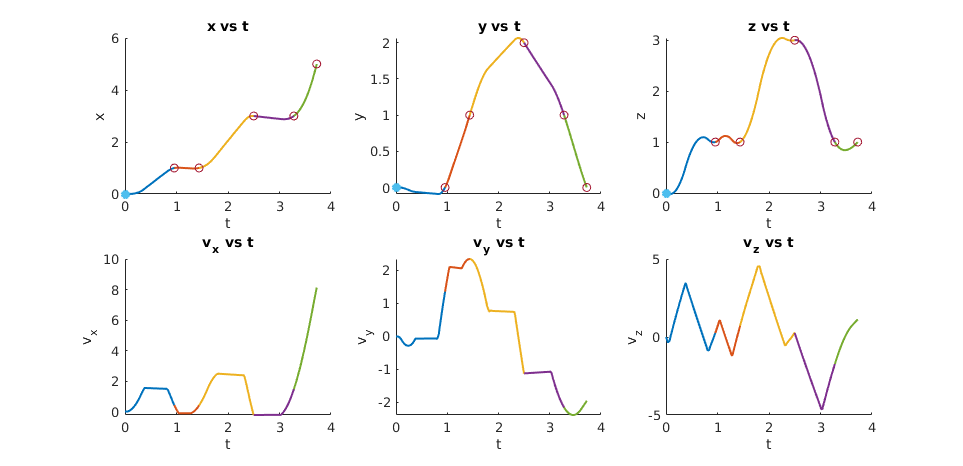
\includegraphics[width=1.0\linewidth]{Images/final_race/pos_vel.png}
	\caption{Position and velocity plot of the complex experiment}
	\label{fig:final_pos_vel}
\end{figure}
\begin{figure}[!htpb]
	\centering
	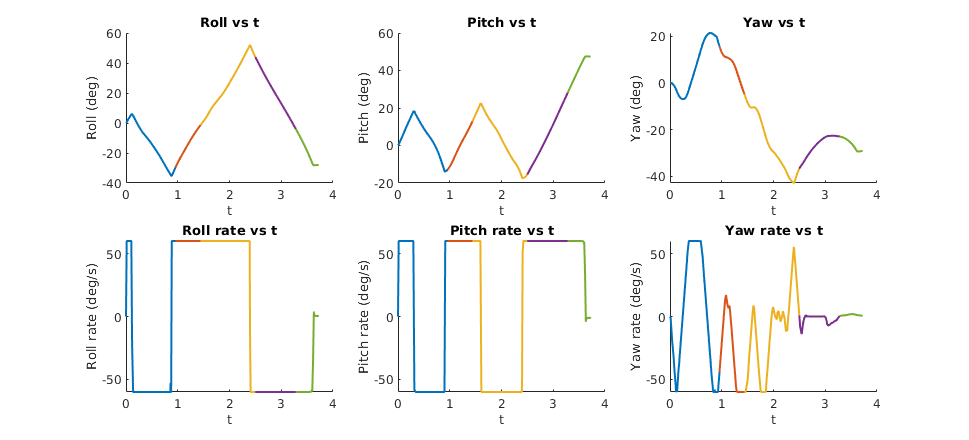
\includegraphics[width=1.0\linewidth]{Images/final_race/orient_rates.png}
	\caption{Orientation and angular rates plot of the complex experiment}
	\label{fig:final_orient_rates}
\end{figure}
\begin{figure}[!htpb]
	\centering
	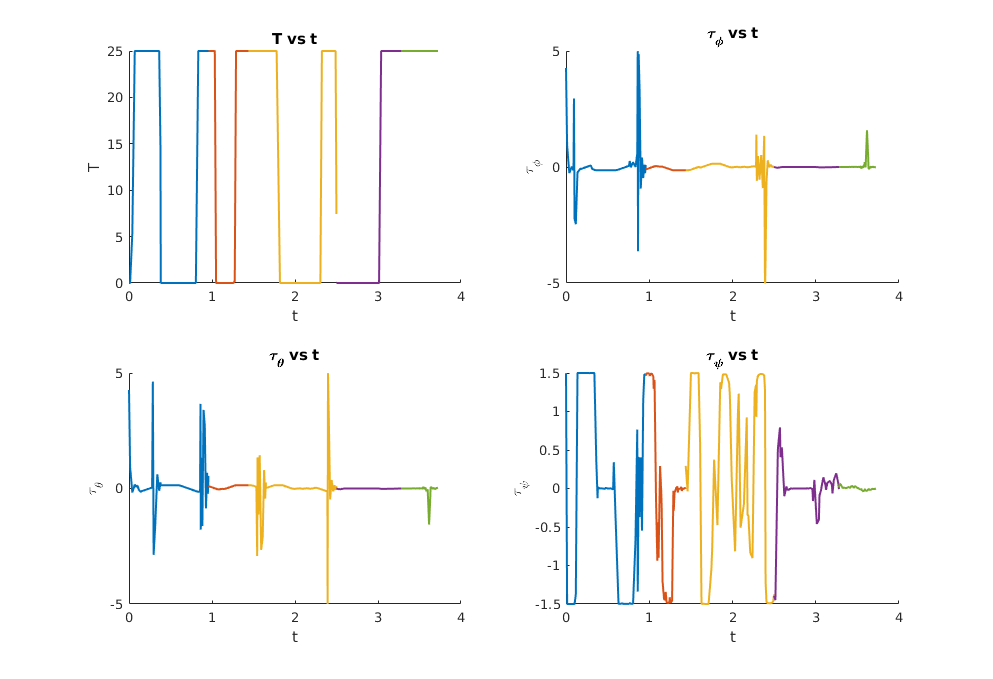
\includegraphics[width=1.0\linewidth]{Images/final_race/controls.png}
	\caption{Control inputs plot of the complex experiment}
	\label{fig:final_controls}
\end{figure}

A video of the drone performing this race was recorded using the procedure explained in Subsection~\ref{subs:video} and it can be found in https://bit.ly/2E2CDAV

\section{CONCLUSIONS}\label{s:conclusions}

Copy abstract... Future work could impose additional gate constraints such as limiting the velocity to a cone, although this constraint is not noticeable if the gates are positioned one (more or less) in front of the other as would happen in a real race.

\addtolength{\textheight}{-12cm}   % This command serves to balance the column lengths
                                  % on the last page of the document manually. It shortens
                                  % the textheight of the last page by a suitable amount.
                                  % This command does not take effect until the next page
                                  % so it should come on the page before the last. Make
                                  % sure that you do not shorten the textheight too much.

%%%%%%%%%%%%%%%%%%%%%%%%%%%%%%%%%%%%%%%%%%%%%%%%%%%%%%%%%%%%%%%%%%%%%%%%%%%%%%%%
%%%%%%%%%%%%%%%%%%%%%%%%%%%%%%%%%%%%%%%%%%%%%%%%%%%%%%%%%%%%%%%%%%%%%%%%%%%%%%%%
%%%%%%%%%%%%%%%%%%% CHECK BIB MANUAL %%%%%%%%%%%%%%%%%%%%%%%%%%%%%%%%%%%%%%%%%%%%%%%%%%%%%%%%%%%%%%%%%
%\begin{thebibliography}{99}

\balance

\makeatletter
\def\endthebibliography{%
	\def\@noitemerr{\@latex@warning{Empty `thebibliography' environment}}%
	\endlist
}
\makeatother

\bibliographystyle{unsrt}
\bibliography{IEEEexample}
%\end{thebibliography}
%%%%%%%%%%%%%%%%%%%%%%%%%%%%%%%%%%%%%%%%%%%%%%%%%%%%%%%%%%%%%%%%%%%%%%%%%%%%%%%%%%%%%%%%%%%%%%%%%%%%%%

\end{document}
